\textit{The program is not done yet; when it is, we will expand this section.}

In this section, we will present the resulting program.

\begin{figure}
  \begin{center}
    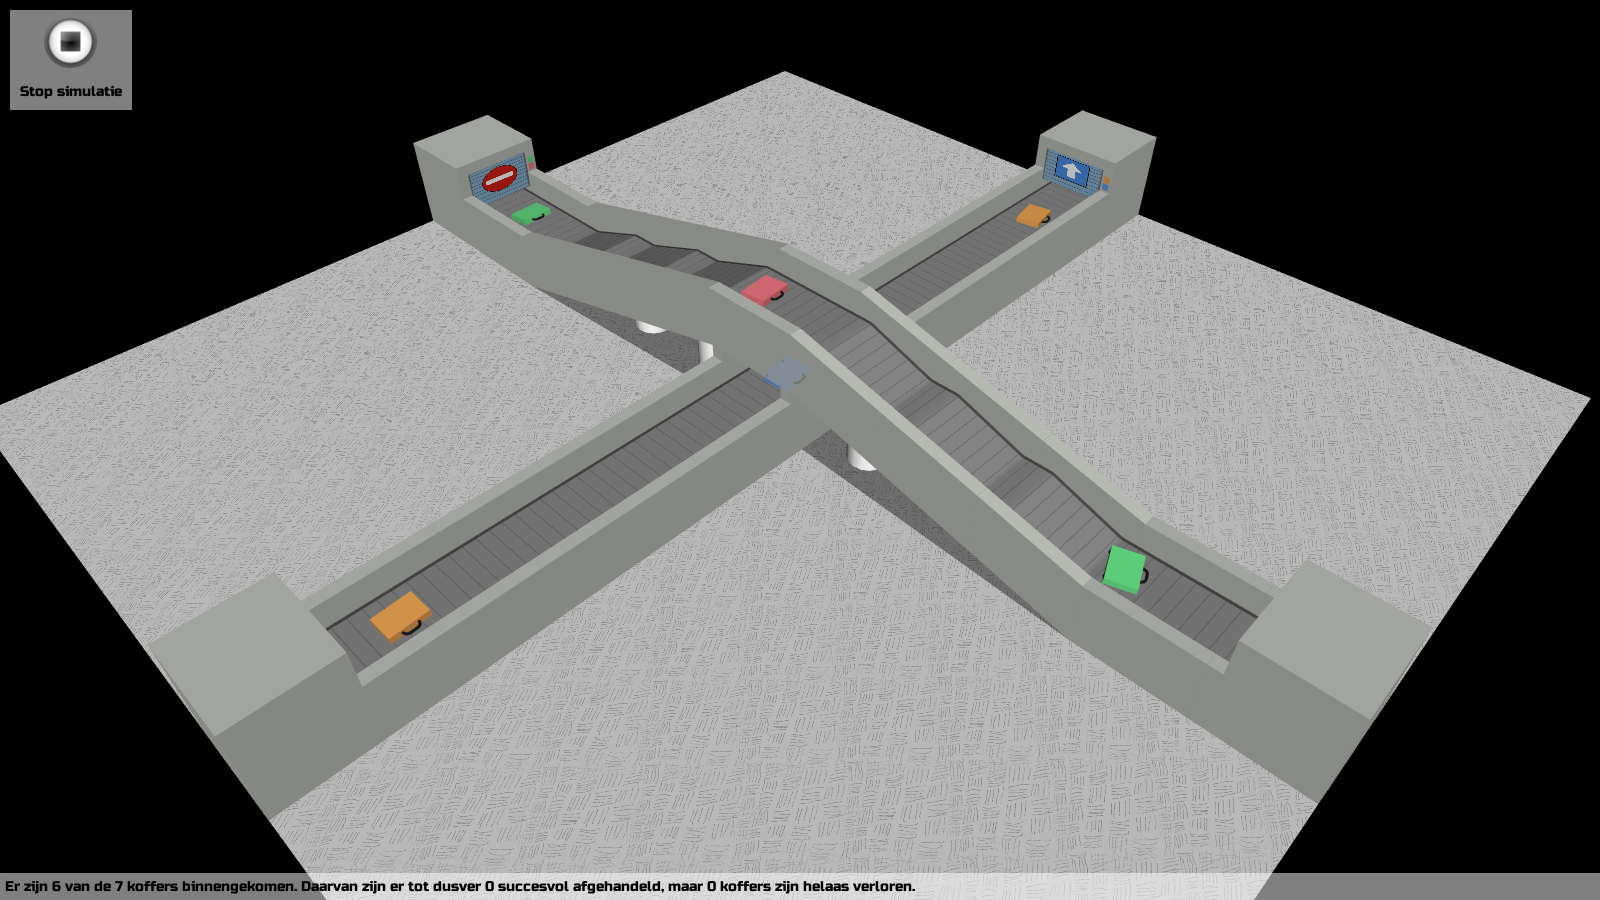
\includegraphics[width=\linewidth]{simulation}
    \caption{Screenshot of the program, showing a running simulation.}
    \label{fig:simulation}
  \end{center}
\end{figure}

\begin{figure}
  \begin{center}
    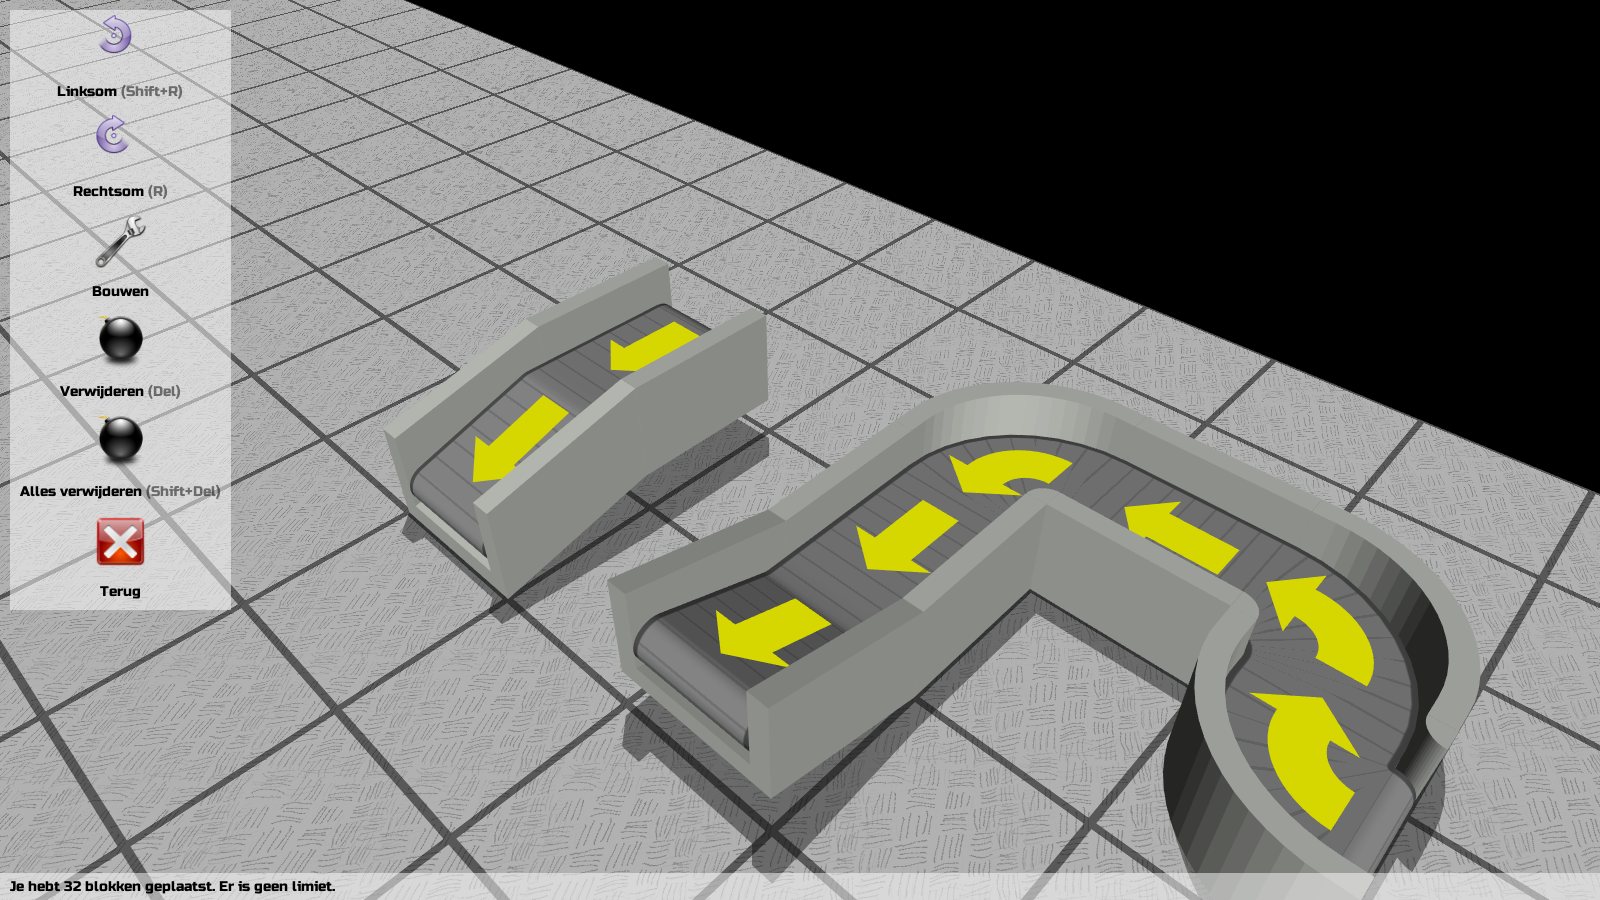
\includegraphics[width=0.7\linewidth]{drawing-together}
    \caption{Adjacent conveyor belts are drawn together as one large conveyor belt.}
    \label{fig:drawing-together}
  \end{center}
\end{figure}

\begin{figure}
  \begin{center}
    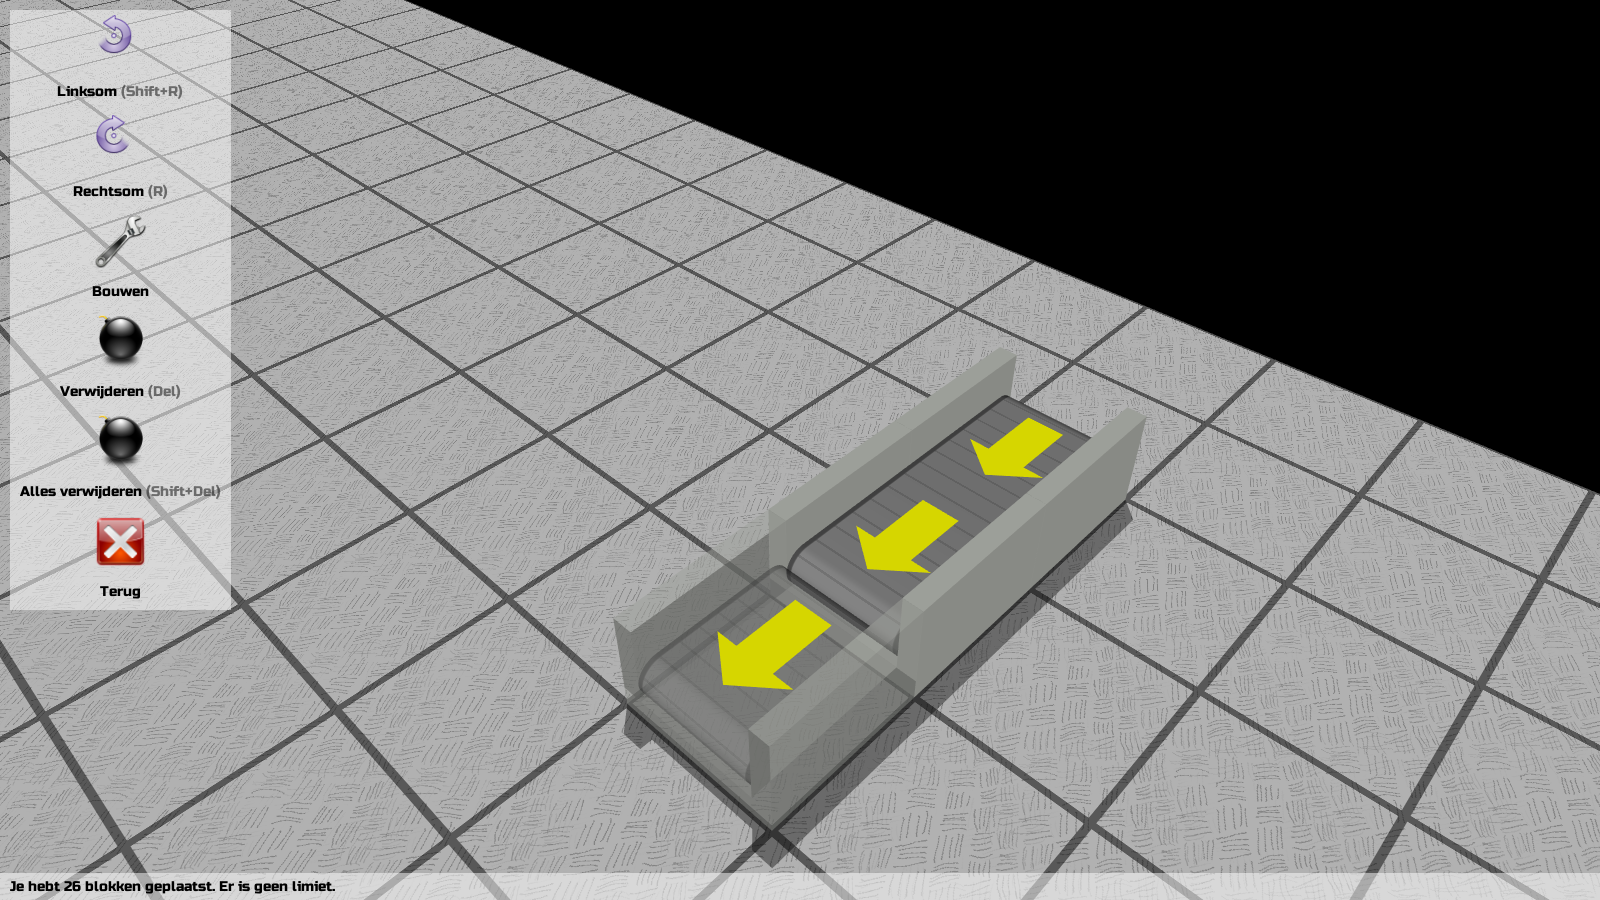
\includegraphics[height=0.3\linewidth]{shadow-block-1}
    \quad
    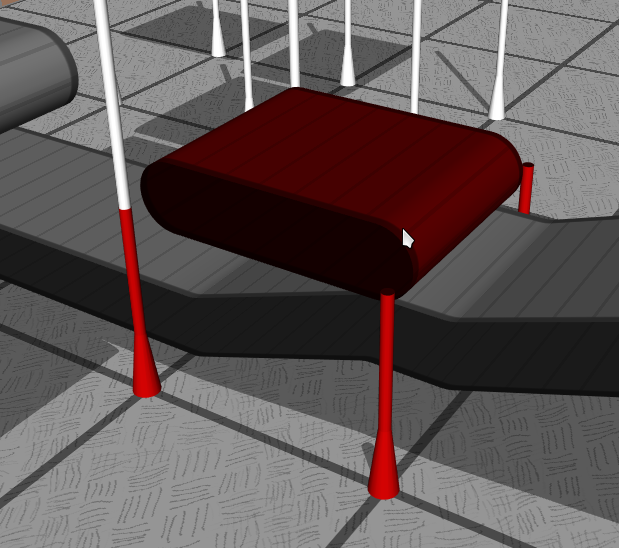
\includegraphics[height=0.3\linewidth]{shadow-block-2}
    \caption{Adding a new block. \textit{Left:} The block that is going to be added is shown as a ``ghost block'' under the cursor. \textit{Right:} If it is not possible to place the block on the indicated location, the ghost block becomes red to show this.}
    \label{fig:shadow-block}
  \end{center}
\end{figure}

\subsection{To be done}
There are quite some tasks that still need to be done.
\begin{itemize}
 \item Drawing more details for the conveyor belts.
 \item Drawing arrows to show the direction of conveyor belts in the building mode. More general, giving more clues to the user what to do (arrows, et cetera).
 \item Being able to choose an existing block to start from.
 \item Improvements to the graphical interface.
 \item Adding scanner blocks.
 \item Making the program more like a game, for example by adding levels and a scoring system.
\end{itemize}
